\documentclass[10pt,letterpaper]{article}
\usepackage[english]{babel}
\usepackage{graphicx}
\usepackage[margin=2cm]{geometry}

\usepackage{subcaption}
\usepackage{mathtools}
\usepackage{amsfonts}
\usepackage{amsmath}
\usepackage{amssymb}
\usepackage{amsthm}
\newcommand{\dif}[1][]{\mathrm{d} {#1}\,}
\newcommand{\rb}[1]{ \left(  {#1} \right) }
\newcommand{\frb}[1]{ \left(  {#1} \right) }

% \usepackage[amsmath,thmmarks,standard]{ntheorem}
\usepackage{comment}
\newtheoremstyle{break}
{\topsep}
{\topsep}%
{\normalfont}
{}%
{\bfseries}
{}%
{\newline}
{}%
\theoremstyle{break}
\newtheorem{exercise}{Exercise}
\newtheorem*{information}{Information}
\newtheorem{mysolution}{Solution}
% \newenvironment{solution}{\begin{comment}}{\end{comment}}
\newtheorem*{mysolutioninformation}{Solution Information}

\usepackage{comment}
% Switch between showing and hiding solutions by commenting out either of the following lines
% \newenvironment{solution}{\begin{mysolution}}{\end{mysolution}} \newenvironment{solutioninformation}{\begin{mysolutioninformation}}{\end{mysolutioninformation}}
\excludecomment{solution} \excludecomment{solutioninformation}






\begin{document}

\title{Characteristics and Weak solutions}
\date{}
\author{}

\maketitle


















\begin{solutioninformation}
	Before we begin to understand the solutions for the exercises in this problem sheet,
	we first briefly describe the method of characteristics for solving non-linear first-order partial differential equations.
	To keep the discussion concise, we forgo the rigorous arguments, although,
	the arguments presented can be made rigorous (for details see the literature references below.).

	Let us consider the following PDE
	\begin{gather} \label{cmPDE}
		\dfrac{du}{dt}+b\frb{x,t,u} \dfrac{du}{dx}=c\frb{x,t,u}, \quad x \in \mathbb{R}, t \in \mathbb{R}^+
	\end{gather}
	with an initial condition
	\begin{gather} \label{cmIC}
		u(x,0)=u_0(x)\ .
	\end{gather}
	While this is not the most general setup the method can treat, it is general enough for our purpose.
	The main idea of the method of characteristics is to find curves in the $x-t$ plane, along which the PDE reduces to an appropriate system of first-order ODEs. These curves are also known as \textit{characteristics}. 

	For a fixed x-intercept $\xi$, consider the following ODE
	\begin{gather} \label{charODE}
		\dfrac{dx}{dt} =b\frb{x,t,u}
		\quad
		x(0) = \xi.
	\end{gather}
	Under sufficient regularity conditions, one can find a unique solution of \eqref{charODE} as $\hat x (\xi,t) = x(t;\xi)$ (parameterized by the initial x-intercept). Thus, along the curve $\{\hat x (\xi,t), t\}$, the PDE \eqref{cmPDE} reduces to the following ODE
	\begin{gather} \label{mainODE}
		\dfrac{d}{dt}\hat u \frb{\xi,t}=c\frb{\hat x,t,\hat u} \quad \hat u\frb{\xi,0}=u_0\frb{\xi},
	\end{gather}
	where $\hat u(\xi,t) = u( \hat x(\xi,t),t) = u( x(t;\xi),t)$. Again, under sufficient regularity conditions we can find a unique solution for \eqref{mainODE}.

	Finally, we need to express the solution in terms of the $(x,t)$. In order to do this, we need to solve for $\xi$ from the equation $x = \hat x\frb{\xi,t}$, i.e., we need to find a smooth function $\hat \xi=\hat \xi(x,t)$ such that
	\begin{gather} \label{xxi}
		x=\hat x\frb{\hat \xi(x,t),t}.
	\end{gather}
	The existence of a function $\hat \xi(x,t)$ satisfying \eqref{xxi} is ensured if $\hat x_\xi\ne0$, due to the inverse function theorem. Thus, the solution to \eqref{cmPDE},\eqref{cmIC} is given by
	\begin{gather} \label{cmSol}
		u(x,t)=\hat u\frb{\hat \xi(x,t) ,t}.
	\end{gather}
	Let us now return to the exercise, where we work with conservation laws of the form:
	\begin{gather} 
		\dfrac{du}{dt}+\dfrac{d f(u)}{dx}=0.
	\end{gather}
\end{solutioninformation}

\begin{exercise}
	The partial differential equation 
	\begin{gather}
		u_t+f(u)_x=0\ ,
		\quad
		u(x,0)=u_0(x)
	\end{gather}%
	with $f(u)=u^2/2$ is known as (the inviscid) Burgers equation. Draw the characteristics of the solution in the $x$-$t$ plane, driven by the initial condition
	\begin{gather} \label{inCond1}
		u(x,0)=
		u_0(x):=\begin{cases}
				0 	&   x< -1
				\\
				1+x & -1 < x<0
				\\
				1-x &  0 < x<1
				\\
				0 	&  1 < x
			\end{cases}\ .
	\end{gather}
	Compute the exact solution in $0<t<1$ and draw its profile at $t=1$.
\end{exercise}

\begin{solution}
	The second exercise requires us to solve \eqref{conLaw} with $f(u)=u^2/2$ and the initial condition
	\begin{gather}
		u_0(x)=\begin{cases}
				0 	& 	  x<-1\\
				1+x  	& -1 < x<0\\
				1-x 	&  0 < x<1\\
				0 	&  1 < x
			\end{cases}\ .
	\end{gather}
	Wherever the solution is smooth, we can write
	\begin{gather}
		\dfrac{du}{dt}+u\dfrac{du}{dx}=0\ .
	\end{gather}
	This PDE has the form \eqref{cmPDE}, with $b(x,t,u) = u$ and $c(x,t,u) = 0$.
	The characteristics are given as the solutions of the ODE
	\begin{gather}
		\dfrac{dx}{dt} =\hat u, 
		\quad
		\dfrac{d\hat u}{dt} = 0,
	\end{gather}
	satisfying the initial conditions
	\begin{gather}
		\hat x\frb{\xi,0} = \xi,
		\quad
		\hat u\frb{\xi,0} =u_0\frb{\xi}.
	\end{gather}
	Since $\hat u$ is clearly constant along the characteristics, we have $\hat u\frb{\xi,t}=u_0\frb{\xi}$.
	Substituting this into the ODE for $\hat x$, we get
	\begin{gather}
		\hat x\frb{\xi,t}=u_0\frb{\xi}t+\xi \ .
	\end{gather}
	It follows that
	\begin{gather}
		\hat x\frb{\xi,t}=\begin{cases}
				\xi 	& 	  \xi<-1\\
				\rb{1+\xi}t+\xi  	& -1 < \xi<0\\
				\rb{1-\xi}t+\xi 	&  0 < \xi<1\\
				\xi 	&  1 < \xi
			\end{cases}\ .
	\end{gather}
	Figure \ref{carXTplane} shows the characteristic curves in the $x$-$t$ plane and the mapping $\xi\mapsto \hat x\frb{\xi,t}$.
	
	To write the solution $u=u(x,t)$ we must first write $\xi$ as a function of $x$ and $t$.
	As Figure \ref{carXTplane} illustrates, this is possible in $0<t<1$, since in that time interval the characteristics do not cross.
	The problem with characteristic curves crossing is that this means that some values of $\xi$ (in our example $0<\xi<1$) correspond to the same value of $x$ at a given time.
	This implies that the map $\xi\mapsto \hat x\frb{\xi,t}$ is not surjective, and therefore can not be inverted.
	\begin{figure}
	\centering
	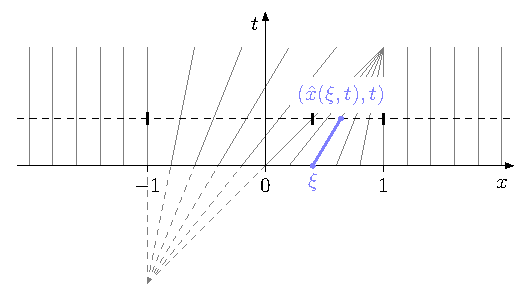
\includegraphics{figures01/charac_t} 
	\caption{The characteristic curves (gray lines) in the $x$-$t$ plane and the map $\xi\mapsto \hat x\frb{\xi,t}$. The dashed gray lines are for illustration.}
	\label{carXTplane}
	\end{figure}
	
	For $0<t<1$ however, we can invert $x=\hat x\frb{\xi,t}$.
	In this example, the way to do this is to fix some $0<t<1$.
	The dashed black line in Figure \ref{carXTplane} corresponds to such a choice.
	Looking at this line we see that $x<-1$, corresponds to characteristics originating in $\xi<-1$, $-1<x<t$ corresponds to $-1<\xi<0$, $t<x<1$ corresponds $0<\xi<1$ and $1<x$ corresponds $1<\xi$.
	Thus,
	\begin{gather}
		\hat \xi(x,t)=\begin{cases}
				x 	& 	  x<-1\\
				\frac{x-t}{1+t}  	& -1 < x<t\\
				\frac{x-t}{1-t} 	&  t< x<1\\
				x 	&  1 < x
			\end{cases}\ .
	\end{gather}
	With similar arguments we find that the solution $u$, in $0<t<1$, is given by
	\begin{gather}
		u(x,t)=u_0\frb{\hat\xi(x,t)}=
			\begin{cases}
				0 	& 	  x<-1\\
				\frac{1+x}{1+t}  	& -1 < x<t\\
				\frac{1-x}{1-t} 	&  t< x<1\\
				0 	&  1 < x
			\end{cases}\ .
	\end{gather}
	Figure \ref{u01} shows the solution $u$ at $t=1$, and the initial function $u_0$.
	\begin{figure}
	\centering
	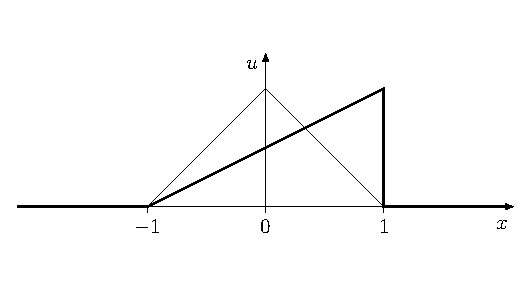
\includegraphics[scale=1]{figures01/usol} 
	\caption{The solution $u$ at $t=1$ (thick line), and the initial function $u_0$ (thin line).}
	\label{u01}
	\end{figure}
\end{solution}





\begin{exercise}
	Consider the following IVP for the Burgers equation
	\begin{gather} \label{Riem}
		u_t+\rb{\frac{u^2}{2}}_x=0
		\quad
		u(x,0)=u_0(x)=\begin{cases}
				u_l & x<0\\
				u_r & 0<x
			\end{cases}\ .
	\end{gather}%
	This is known as a \emph{Riemann problem}. 
	For $u_l<u_r$, and any $u_m\in\rb{u_l,u_r}$, let
	\begin{gather}%
		u(x,t)=\begin{cases}
				u_l & x<s_mt\\
				u_m & s_mt<x<u_mt\\
				x/t & u_mt<x<u_rt\\
				u_r & u_rt<x
			\end{cases}\ ,
	\end{gather}%
	where $s_m=(u_m+u_l)/2$.
	Show that $u$ is a weak solution of \eqref{Riem}, and draw its characteristics.
	Can you give the expression of any other weak solution for this problem?
\end{exercise}

\begin{solution}
	For abbreviation, we use the notation
	\begin{gather}
		B\frb{\phi,u}: =\int_0^\infty \int_{-\infty}^\infty \Big(\phi_t u +\phi_x f(u)\Big)\dif x\dif t\ ,
	\end{gather}
	for any compactly supported $C^1$ function. Thus, we have to show
	\begin{gather} \label{WS}
		B\frb{\phi,u}=-\int_{-\infty}^\infty \phi(x,0)u(x,0)\dif x\ .
	\end{gather}
	Let us consider the Riemann problem for the Burgers equation, with the initial condition
	\begin{gather} 
		u(x,0)=u_0(x)=\begin{cases}
				u_l & x<0\\
				u_r & 0<x
			\end{cases}\ .
	\end{gather}
	For $u_l<u_r$, and any $u_m\in\rb{u_l,u_r}$, we wish to show that
	\begin{gather}
		u(x,t)=\begin{cases}
				u_l & x<s_mt\\
				u_m & s_mt<x<u_mt\\
				x/t & u_mt<x<u_rt\\
				u_r & u_rt<x
			\end{cases}\ ,
	\end{gather}
	satisfies \eqref{WS}. We first define the functions
	\begin{gather}
		u_1(x,t)=\begin{cases}
				u_l & x<s_mt\\
				u_m & s_mt<x
			\end{cases}\ ,
		\quad
		u_2(x,t)=\begin{cases}
				u_m & x<u_mt \\
				x/t & u_mt<x<u_rt\\
				u_r & u_rt<x
			\end{cases}\ ,
	\end{gather}
	and note that
	\begin{gather}
		u(x,t)=u_1(x,t)+u_2(x,t)-u_m\ ,
	\end{gather}
	and
	\begin{gather} \label{fsum}
		f\frb{u(x,t)}=f\frb{u_1(x,t)}+f\frb{u_2(x,t)}-f\frb{u_m}\ .
	\end{gather}
	Thus,
	\begin{gather} \label{Bsum}
		B\frb{\phi,u}=B\frb{\phi,u_1}+B\frb{\phi,u_2}-B\frb{\phi,u_m}\ .
	\end{gather}
	For $B\frb{\phi,u_1}$, consider the change of variables $y = x - s_mt$ and $\tau = t$. Note that we will also need to change the derivatives with respect to $x$ and $t$ to derivatives with respect to $y$ and $\tau$. In other words, for $\widetilde \phi(y,\tau) = \phi(x(y,\tau),t(y,\tau))$, the chain rule gives us
	\begin{align*}
		\widetilde \phi(y,\tau)_t &=\widetilde \phi_y(y,\tau) y_t + \widetilde \phi_\tau(y,\tau) \tau_t\\
		&=
		-s_m \phi_y(y,\tau) + \widetilde \phi_\tau(y,\tau),
	\end{align*}
	\begin{align*}
		\widetilde \phi(y,\tau)_x &=\widetilde \phi_y(y,\tau) y_x + \widetilde \phi_\tau(y,\tau) \tau_x\\
		&= \widetilde \phi_y(y,\tau).
	\end{align*}
	Thus, the integral terms change to
	\begin{gather}
		B\frb{\phi,u_1}=\int_0^\infty \int_{-\infty}^\infty
				\Big( \left[ \widetilde \phi_\tau(y,\tau) -s_m \widetilde \phi_y(y,\tau)\right] u_1\frb{y+s_m \tau, \tau} + \widetilde \phi_y(y,\tau)  f(u_1\frb{y+s_m \tau, \tau}) \Big)
			J \dif y\dif \tau\ 
	\end{gather}
	where
	\begin{gather}
		J = \text{Det} \left( \frac{\partial(x,t)}{\partial(y,\tau)} \right) = 1.
	\end{gather}
	The integral simplifies to
	\begin{align} \label{Bsum1}
		B\frb{\phi,u_1}&=\int_0^\infty \int_{-\infty}^0
				\Big( \left[ \widetilde \phi_\tau(y,\tau) -s_m \widetilde \phi_y(y,\tau)\right] u_l + \widetilde \phi_y(y,\tau)  \frac{u_l^2}{2} \Big)
			 \dif y\dif \tau\  \\
			 & + \int_0^\infty \int_0^{\infty}
				\Big( \left[ \widetilde \phi_\tau(y,\tau) -s_m  \widetilde\phi_y(y,\tau)\right] u_m + \widetilde \phi_y(y,\tau)  \frac{u_m^2}{2} \Big)
			 \dif y\dif \tau\ \\
			 &= \int_0^\infty \widetilde \phi(0,\tau) \left[(u_m - u_l) s_m + \frac{u_l^2}{2} - \frac{u_m^2}{2} \right] \dif \tau - \int_{-\infty}^{\infty} \left[\widetilde \phi(y,\tau) u_1(y+s_m \tau,\tau) \right]\Big|_{\tau=0} \dif y\\
			 &= - \int_{-\infty}^{\infty} \phi(x,0) u_1(x,0) \dif x.
	\end{align}
	Next, let us consider $B\frb{\phi,u_2}$. Note that the $u_2$ may suffer from a singularity as $t \rightarrow 0^+$. Thus, we isolate the possible singularity using an $1>\epsilon > 0$ by splitting the integral
	\begin{align}
	B\frb{\phi,u_2} &=  \int_0^\epsilon \int_{-\infty}^\infty \Big(\phi_t u +\phi_x f\frb{u_2}\Big)\dif x\dif t +  \int_\epsilon^\infty \int_{-\infty}^\infty \Big(\phi_t u_2 +\phi_x f\frb{u_2}\Big)\dif x\dif t \\
	 & = I_1 + I_2 \ .
	\end{align}
	Since the integrand in $I_2$ is a continuous, we can perform an integration by parts to get
	\begin{align}
	I_2 &= - \int_\epsilon^\infty \int_{u_m t}^{u_r t} \phi(x,t) \left( - \frac{x}{t^2} + \frac{1}{2} \frac{2 x}{t} \right) \dif x \dif t - \int_{-\infty}^\infty \phi(x,\epsilon) u_2(x,\epsilon) \dif x  \\
		& = - \int_{-\infty}^\infty \phi(x,\epsilon) u(x,\epsilon) \dif x.
	\end{align}
	Also, choosing a finite $L>0$ such that $\phi_t$ and $\phi_x$ vanish outside $[-L,L$], we have
	\begin{align}
	|I_1| &\leq \left| \int_0^\epsilon \int_{-L}^{u_mt} \Big(\phi_t u_m +\phi_x \frac{u_m^2}{2}\Big)\dif x\dif t \right| + \left| \int_0^\epsilon \int_{u_mt}^{u_rt} \Big(\phi_t \frac{x}{t} +\phi_x \frac{x^2}{2t^2}\Big)\dif x\dif t \right|  \\
	&+ \left| \int_0^\epsilon \int_{u_rt}^L \Big(\phi_t u_r +\phi_x \frac{u_r^2}{2}\Big)\dif x\dif t \right| \\
	&\leq \max{(\|\phi_t\|_\infty|u_m|,\|\phi_x\|_\infty|u_m^2|)} \left( \frac{|u_m| \epsilon^2}{2} + L \epsilon \right) \\
	& + \max{\big(\|\phi_t\|_\infty \max(|u_m|,|u_r|),\|\phi_x\|_\infty \max(|u_m^2|,|u_r^2|)\big)} (u_m - u_r) \epsilon^2 \\
	& + \max{(\|\phi_t\|_\infty|u_r|,\|\phi_x\|_\infty|u_r^2|)} \left( \frac{u_r \epsilon^2}{2} + L \epsilon \right) \\
	& \leq C(u_l,u_r, u_m, \phi) \epsilon
	\end{align}
	where $C$ is independent of $\epsilon$. Thus, $I_1 \rightarrow 0$ as $\epsilon \rightarrow 0^+$ and
	\begin{gather} \label{Bsum2}
		B\frb{\phi,u_2}= - \lim \limits_{\epsilon \rightarrow 0^+} I_2 = \int_{-\infty}^{\infty} \phi(x,0) u_2(x,0) \dif x\ .
	\end{gather}
	Finally, 
	\begin{gather} \label{Bsumm}
		B\frb{\phi,u_m}= - \int_{-\infty}^{\infty} \phi(x,0) u_m \dif x\ .
	\end{gather}
	Using \eqref{Bsum1}, \eqref{Bsum2} and \eqref{Bsumm} we get the required result.
\end{solution}





\begin{exercise}
	In this example the flux $f$ depends on $x$ as well as on the solution $u$.
	Suppose $u$ is the solution of the PDE
	\begin{gather}%
		u_t +\rb{a(x)u}_x=0,
		\quad
		a(x)= x
	\end{gather}%
	which satisfies the initial condition $u(x,0)=u_0(x)$, where $u_0$ is some given smooth function.
	Use the method of characteristics to compute the equation describing the characteristics in the $x$-$t$ plane.
	Is the solution $u$ constant on the characteristic curves?
\end{exercise}

\begin{solution}
	Suppose $u$ satisfies
	\begin{gather}
		\dfrac{du}{dt}+\dif{}{x}\rb{a(x)u}=0
		\quad
		a(x)=x
	\end{gather}
	and the initial condition $u(x,0)=u_0(x)$, where $u_0$ is some given smooth function.
	In a neighborhood of the initial condition,
	\begin{gather}
		\dfrac{du}{dt}+x \dfrac{du}{dx}=-u\ ,
	\end{gather}
	therefore, the characteristics are given by the IVP
	\begin{gather} \label{charSin}
		%TODO
		=x
		\quad
		\hat x\frb{\xi,0}=\xi\ .
	\end{gather}
	The solution $\hat x$ to the ODE in \eqref{charSin} is obtained fas
	\begin{gather}
		\hat x\frb{\xi,t}=\xi e^t\ .
	\end{gather}
	The IVP for $u$ on the characteristics is
	\begin{gather}
		\dfrac{d\hat u}{dt}=-u
		\quad
		\hat u\frb{\xi,0}=u_0\frb{\xi}\ .
	\end{gather}
	which has the solution $\hat u(\xi,t) = u_0(\xi) e^{-t}$. Thus, $u$ is not constant on the characteristics, unless $u_0$ is identically zero.	
\end{solution}









% \begin{exercise}
%     Find the characteristics associated with the transport problem 
%     $$
%         \partial_t u(x,t) + \partial_x\left( (-x) u(x,t) \right) = 0,
%     $$
%     where the speed is $a(x) = -x$.
%     Draw a few examples for these curves. 
%     Solve the characteristic equation for some initial value $u_0$.
% \end{exercise}
% \begin{solution}
%     The characteristic curve starting at $x_0$ obeys the ordinary differential equation 
%     \begin{align*}
%         \partial_t x(t) = - x(t), \quad x(0) = x_0.
%     \end{align*}
%     We know that the solution is 
%     \begin{align*}
%         x(t) = x_0 \exp(-t).
%     \end{align*}
%     As in the lecture, we derive the following ordinary differential equation 
%     for the values of $u$ along the characteristic curve emanating at $x_0$: 
%     \begin{align*}
%         \partial_t v(t) = - \partial_x a( x(t) ) v(t), \quad v(0) = u_0( x(0) ), 
%     \end{align*}
%     that is, 
%     \begin{align*}
%         \partial_t v(t) = x(t) v(t), \quad v(0) = u_0( x(0) ), 
%     \end{align*}
%     We remember (or look up) the solution formula for this ordinary differential equation:
%     \begin{align*}
%         v(t) = u_0(x_0) \cdot e^{\int_0^t x(s) \;ds + x_0}.
%     \end{align*}
%     With our specific formula for $x(t)$, this gives 
%     \begin{align*}
%         v(t) 
%         &
%         = 
%         u_0(x_0) \cdot e^{x_0 \int_0^t \exp(-s) \;ds + x_0}
%         = 
%         u_0(x_0) \cdot e^{ - x_0 e^{-t} + x_0}
%         = 
%         u_0(x_0) \cdot e^{ x_0 ( 1 - e^{-t} ) }
%         .
%     \end{align*}
%     \textit{Remark: 
%     The interpretation of this system is that we have a transport towards the origin.
%     Each characteristic curve goes flat very quickly,
%     since the speed goes to zero as we approach the origin. 
%     }
% \end{solution}





\begin{information}
	A function $u$ is said to be a \emph{weak solution} to the initial value problem (IVP)
	\begin{gather} \label{conLaw}
		u_t+f(u)_x=0\ ,
		\quad
		u(x,0)=u_0(x)
	\end{gather}%
	if for any compactly supported $C^1$ function $\phi=\phi(x,t)$, there holds
	\begin{gather}%
		\int_0^\infty \int_{-\infty}^\infty \Big( \phi_t u +\phi_x f(u)\Big)\dif x\dif t
		=
		-\int_{-\infty}^\infty \phi(x,0)u_0(x)\dif x\ .
	\end{gather}%
\end{information}



\begin{exercise}
	Suppose $f\!\left(u\right)=au$, where $a>0$ is a constant and $u_{0}\!\left(x\right)$ is an integrable function. Verify that $u(x)=u_{0}(x-at)$ satisfies \eqref{conLaw} in integral form:
	\begin{gather} \label{weakForm}
		\int_{x_{1}}^{x_{2}}u\!\left(x,t_{2}\right) dx
		-
		\int_{x_{1}}^{x_{2}}u\!\left(x,t_{1}\right)dx
		=
		-
		\int_{t_{1}}^{t_{2}}f\!\left(u\!\left(x_{2},t\right)\right)dt
		+
		\int_{t_{1}}^{t_{2}}f\!\left(u\!\left(x_{1},t\right)\right)dt 
		\ .
	\end{gather}%
\end{exercise}

\begin{solution}
	The integral form of the scalar conservation law \eqref{conLaw} is given by 
	\begin{gather} 
		\int_{x_{1}}^{x_{2}}u\frb{x,t_{2}} \dif x
				-\int_{x_{1}}^{x_{2}}u\frb{x,t_{1}} \dif x
			=-\int_{t_{1}}^{t_{2}}f\frb{u\frb{x_{2},t}} \dif t
				+\int_{t_{1}}^{t_{2}}f\frb{u\frb{x_{1},t}} \dif t\ .
	\end{gather}
	For $f(u)=au$, the conservation law is reduced to the advection equation. Substituting $f\!\left(u\right)=au$ into (\ref{weakForm}) yields
	\begin{gather} \label{AdvecIntForm}
		\int_{x_{1}}^{x_{2}}u\frb{x,t_{2}} \dif x
				-\int_{x_{1}}^{x_{2}}u\frb{x,t_{1}} \dif x
			=-a \int_{t_{1}}^{t_{2}} u\frb{x_{2},t} \dif t
				+a\int_{t_{1}}^{t_{2}} u\frb{x_{1},t} \dif t\  .
	\end{gather}
	On the left hand side of \eqref{AdvecIntForm} is an integral in $x$, and on the right hand side is an integral in $t$.
	
	Let $u_{0}(x)$ be any integrable function, i.e., $u_{0}(x)$ may include discontinuities. If $u(x,t)=u_0(x-at)$, then the left hand side and ride hand side of \eqref{AdvecIntForm} take the form
	\begin{gather} \label{LHS}
		LHS=\int_{x_{1}}^{x_{2}}u_{0}\frb{x-at_{2}}\dif x
				-\int_{x_{1}}^{x_{2}}u_{0}\frb{x-at_{1}} \dif x,
	\end{gather}
	\begin{gather} \label{RHS}
		RHS=-a\int_{t_{1}}^{t_{2}}u_{0}\frb{x_{2}-at}\dif t
				+a\int_{t_{1}}^{t_{2}}u\frb{x_{1}-at}\dif t\ 
	\end{gather}
	respectively. By substituting the integration variable $y=x-at_{2}$ into the first integral of \eqref{LHS}, and the integration variable $y=x-at_{1}$ into the second, we get
	\begin{gather} \label{LHS2}
		LHS=\int_{x_{1}-at_{2}}^{x_{2}-at_{2}}u_{0}\frb{y}\dif y
			-\int_{x_{1}-at_{1}}^{x_{2}-at_{1}}u_{0}\frb{y}\dif y\ .
	\end{gather}
	Similarly, by substituting $y=x_{2}-at$ into the first integral of \eqref{RHS}, and $y=x_{1}-at$ in the second we get 
	\begin{gather} \label{RHS2}
		RHS=- \int_{x_{2}-at_{2}}^{x_{2}-at_{1}}u_{0}\frb{y}\dif y
			+\int_{x_{1}-at_{2}}^{x_{1}-at_{1}}u_{0}\frb{y} \dif y\ .
	\end{gather}
	Subtracting \eqref{RHS2} from \eqref{LHS2}, we get
	\begin{gather}
		LHS-RHS=\int_{x_{1}-at_{2}}^{x_{2}-at_{1}}u_{0}\frb{y} \dif y
			-\int_{x_{1}-at_{2}}^{x_{2}-at_{1}}u_{0}\frb{y} \dif y=0\ ,
	\end{gather}
	from which we conclude that for any integrable function $u_{0}\!\left(x\right)$, $u\!\left(x,t\right)=u_{0}\text{\!}\left(x-at\right)$ is a solution to the advection equation on integral form.
\end{solution}
	



\begin{thebibliography}{----}
	\bibitem{Evans}
	\newblock{Partial Differential Equations}, by Lawrence. C. Evans.
	\newblock{\em Chapter 3, Section 2}.
	
	\bibitem{Fritz}
	\newblock{Partial Differential Equations}, by Fritz John.	
\end{thebibliography}


\end{document}
